\documentclass[12pt, a4paper]{article}

\usepackage{booktabs}
\usepackage{graphicx}
\usepackage{hyperref}
\usepackage[margin=0.8in]{geometry} %set page margins
\usepackage{array} % needed for m column type in tabular
\usepackage[capitalise]{cleveref}

\usepackage{fancyhdr}
\pagestyle{fancy}
\setlength{\headheight}{28pt}

\fancyhead[L]{\myauthor}
\fancyhead[R]{\mydate}
\fancyhead[C]{\mytitle}

\fancyfoot[C]{\thepage}
\fancyfoot[L,R]{}
\renewcommand{\headrulewidth}{0.4pt}
\renewcommand{\footrulewidth}{0.4pt}

\newcommand{\mytitle}{Postcode Anonymity Analysis} %redefine these hear as they get wiped by \maketitle 
\newcommand{\mydate}{May 2021}
\newcommand{\myauthor}{Adam Hardy}
\title{\mytitle}
\author{\myauthor}
\date{\mydate}

\begin{document}
\maketitle

\section{Introduction}

In the US, 5-digit Zip codes are usually rounded to 3-digits when anonymising healthdata, so knowledge of the Zip code doesn’t allow small groups to be identified.  Even then, there are some 3-digit codes that have fewer than 20,000 residents, and the advice is to lump these together under a new code (000). Looking forward to how GDPR may affect data handling in the UK, is it possible to use a similar approach here?

UK postcodes can be in one of six formats and broken down into seven componenets that describe geographic areas (\cref{table:postcode_format}). Given how UK postcodes are constructed, we can`t simply truncate postcodes to three characters as is done for USA zip codes as this will result in postcode areas being combined together in ways which do not have real geographic meaning. For example, `NE3 1ED' and `NE35 2FG' are both valid postcodes. Truncating both of these to the first three characters would put these both in the `NE3' group. They should instead both be in an `NE' area group or separate `NE3' and `NE35' district groups (or another chosen postcode component group).

Below, we take a UK postcode and population dataset\footnote{\url{http://www.nomisweb.co.uk/output/census/2011/Postcode_Estimates_Table_1.csv}} and perform an anonymity analysis of the postcode geographic components on the four population groups present in the dataset: total population, male population, female population and occupied households.

\begin{table}
\begin{center}
	\begin{tabular}{ m{0.125\textwidth}  m{0.1\textwidth}  m{0.1\textwidth}  m{0.07\textwidth}  m{0.1\textwidth}  m{0.1\textwidth}  m{0.1\textwidth}  m{0.07\textwidth}}
		\toprule
        Postcode Format & Outward Code & Inward Code & Area & District & Sub-District & Sector & Unit \\
        \midrule
		AA9A 9AA & AA9A & 9AA & AA & AA9 & AA9A & AA9A 9 & AA \\
        A9A 9AA & A9A & 9AA & A & A9 & A9A & A9A 9 & AA \\
        A9 9AA & A9 & 9AA & A & A9 & \textbf{\textbf{N/A}} & A9 9 & AA \\
        A99 9AA & A99 & 9AA & A & A99 & \textbf{N/A} & A9 9 & AA \\
        AA9 9AA & AA9 & 9AA & AA & AA9 & \textbf{N/A} & AA9 9 & AA \\
        AA99 9AA & AA99 & 9AA  & AA & AA99 & \textbf{N/A} & AA99 9 & AA\\
        \bottomrule
    \end{tabular}
\caption{UK postcode formats and geographic components. `A' represents an alphabetic character, `9' represent a numeric character. Obtained from \url{https://ideal-postcodes.co.uk/guides/uk-postcode-format}.}\label{table:postcode_format}
\end{center}
\end{table}

\section{Anonymity Analysis}
\subsection{Anonymity Threshold}

For our anonymity analysis we are most concerned about small groups, as they are most likely to contain non-anonymous data. We will use an anonymity threshold, which is the smallest group size that would be acceptable in an anonymised dataset.

 The number of groups which are smaller than threshold gives us a measure of how well a chosen combination of postcode component and population group anonymises the data. It is of course possible to aggregate small groups into larger ones, but this is best done when the majority of groups are already anonymised.

\subsection{Postcode Component Selection}

We have used the area, district, sub-district and and sector components of the postcode; these represent increasingly smaller geographic areas, with the full postcode being the smallest. Where a postcode does not have a sub-district (the sub-district is mostly used in areas of London), we have substituted the district in its place.

In~\cref{fig:postcode_selection} we have plotted the percentage of of groups below the anonymity threshold, against the anonymity threshold for each postcode component and population group. Where the percentage of groups below the threshold is low, this means that the data would be well anonymised and vice versa. To use these plots:
\begin{enumerate}
\item Choose the population of interest.
\begin{itemize}
\item For example, the total population (top left graph)
\end{itemize}
\item Select an anonymity treshold on the x-axis. 
\begin{itemize}
\item This threshold should be chosen so that data is considered anonymised if all the geographic postcode groups are larger than the threshold
\item i.e.\ a treshold of $10{^5}$ means that data is considered anonymous if the smallest group size is larger than 100,000.
\end{itemize}
\item The value of the curve at the chosen threshold tells you what percentage of groups are smaller than this threshold.
\begin{itemize}
\item e.g.\ for a threshold of $10{^5}$, only a small number the groups at the postcode area level (red curve) are smaller than 10,000 total population.
\item This would probably be considered anonymous at this level, as the remaining small groups can be aggregated into a single larger one.
\item In contrast, at the sector, sub-district of district level, close to 100\% of the groups are below this threshold, and the data would be defined as not anonymous.
\end{itemize}
\end{enumerate}

We see that each curve has a region where it rises very sharply. To the left this steep region it is clear the data would be well anonymised, and to the right it would be poorly anonymised. Within the steep region it is less clear.

\begin{figure}
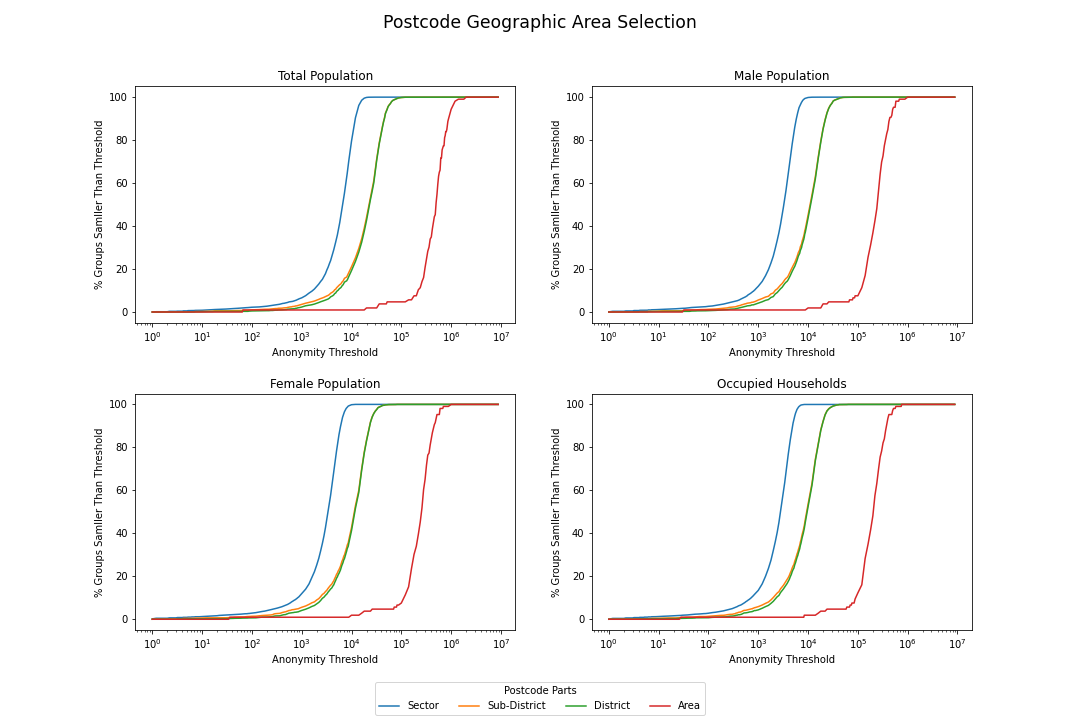
\includegraphics[width=1\textwidth,trim={3cm, 0cm, 3cm, 0cm},clip]{images/postode_selection.png}
\caption{Postcode component selection.}\label{fig:postcode_selection}
\end{figure}

\subsection{Population Segment Selection}

If the postcode geographic component is already chosen, it might be desireable to choose what population level to publish: total population, male \& female or households. Using the same data we can arrange the plots (\cref{fig:population_selection}) to provide a similar utility to the above for this scenario:
\begin{enumerate}
\item Choose the postcode geographic level of interest.
\begin{itemize}
\item For example, the district (bottom left graph)
\end{itemize}
\item Select an anonymity treshold on the x-axis. 
\item The value of the curve at the chosen threshold tells us what percentage of groups are smaller than this threshold.
\begin{itemize}
\item e.g.\ for a threshold of $10^{4}$, about 15\% of groups at the district level are smaller than 10,000 total population (blue curve) and about 35\% of the groups are smaller than the threshold for the remaining population measures.
\end{itemize}
\end{enumerate}
\begin{figure}
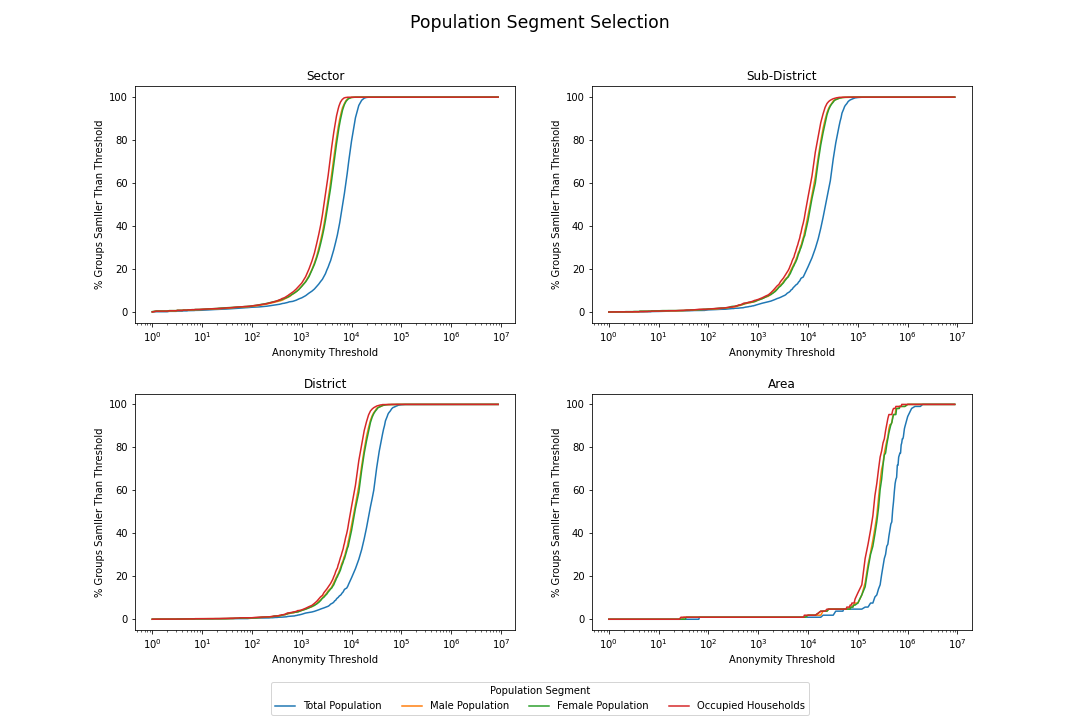
\includegraphics[width=1\textwidth,trim={3cm, 0cm, 3cm, 0cm},clip]{images/population_selection.png}
\caption{population selection}\label{fig:population_selection}
\end{figure}

\section{Lookup Utility}\label{lookup-utlity}

\section{Examples}
\subsection{Example A}
\begin{itemize}
\item Population group: \textit{Total Population}
\item Anonymity threshold: $100,000$
\end{itemize}
Using top right of~\cref{fig:postcode_selection}, we see that all of the district, sub-district and sector group sizes are below the threshold, leaving only area. Using the lookup utility (\cref{lookup-utlity}) we can find that there are 5 postcode areas with a population below the treshold, listed in~\cref{table:example_a}. These five groups could be aggregated into one larger group that would be of size 138,322 - above the anonymity threshold.

\begin{table}
\begin{center}
\begin{tabular}{ll}
    \toprule
    Area &  Total Population \\
    \midrule
    DG   &                65 \\
    TD   &             18,331 \\
    EC   &             33,956 \\
    WC   &             35,745 \\
    LD   &             50,225 \\
    \bottomrule
\end{tabular}
\caption{Postcodes areas below the anonymity threshold for Example A}\label{table:example_a}
\end{center}
\end{table}

\subsection{Example B}

\begin{itemize}
    \item Population group: \textit{Occupied Households}
    \item Anonymity threshold: $1,200$
\end{itemize}

Area would be a confident choice in this case as only a single group is smaller than the selected anonymity threshold. However, if we want to maintain as much information as possible in the dataset, we may want to choose a smaller postcode component. At the sector level $26.2\%$ of groups are smaller than the anonymity threshold. Aggregating all of these into one group (of $\approx770,000$ in size) would leave us with $\approx6,000$ groups, many more than 105 groups we would have at the area level while still having an anonymised dataset.

\section{Summary}



\end{document}